\documentclass[tikz]{standalone}

\usetikzlibrary{automata,positioning}

\begin{document}
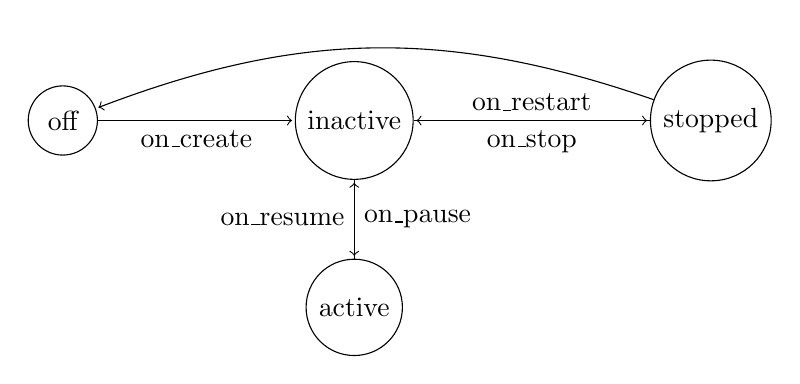
\begin{tikzpicture}[->,shorten >= 1pt,node distance=3cm,auto]
	\node[state] (off)   {off};
	\node[state] (inact) [right=of off,xshift=-0.5cm] {inactive};
	\node[state] (act)   [below=of inact,yshift=2cm] {active};
	\node[state] (back)  [right=of inact] {stopped};
	\path[->]
	(off)   edge [below] node {on\_create} (inact)
	(inact) edge [left]  node {on\_resume} (act)
	        edge [below] node {on\_stop} (back)
	(back)  edge [above] node {on\_restart}  (inact)
	        edge [bend right=20] node {}  (off)
	(act)   edge [right] node {on\_pause}  (inact);
\end{tikzpicture}
\end{document}
